\subsection{Interface}

Ein\textbf{ User Interface (UI)} in eingebetteten Systemen ermöglicht eine Interaktion zwischen Benutzer und Gerät.

Das \textbf{Interface} besteht aus \textbf{Encodern}, \textbf{Schiebepotentiometern}, einem \textbf{LCD-Display }und \textbf{Buttons}. Dessen Zusammenspiel ermöglicht dem Benutzer die nötige Kontrolle über den Sampler.


Im folgenden Kapitel wird Ihnen die Funktionalität, Implementierung, Ansteuerung, sowie das Zusammenspiel der Komponenten untereinander nähergebracht: 

\subsubsection{Encoder}

\textbf{Grundfunktionalität:}


Der \textbf{Encoder} dient der Navigation im Benutzer-Menü des Samplers. Er ermöglicht die Auswahl von Samples und das Scrollen durch die Sample-Liste, die auf dem LCD-Display angezeigt wird. Diese Liste zeigt die Namen der Samples an, die zuvor durch die Fader-Einstellungen bestimmt wurden. Der Cursor an der Seite zeigt die Aktuelle Position des Cursors an. Der Sample gilt als ausgewählt wen dessen Name unter der Liste erscheint.

\textbf{Umsetzung der Funktionalität:}

Die Auswahl von Samples sowie das Inkrementieren und Dekrementieren des Cursors, welcher sich im Struct des Filemanager befindet werden durch Interrupts unterstützt. Wenn der Encoder bewegt oder gedrückt wird, sendet er Signale an die MCU, die Interrupts auslösen.

Die Auswertung dieser Signale erfolgt dann in der Callback  \mintinline{c}|HAL_GPIO_EXTI_Callback(uint16_t GPIO_Pin)|. 

\begin{figure}[H]
	\centering
	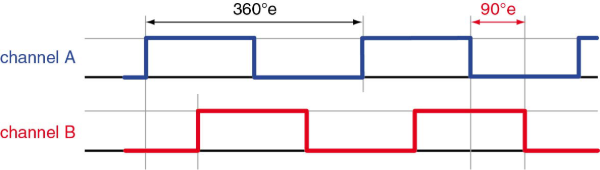
\includegraphics[width=0.8\textwidth]{images/08_durchfuehrung/interface/encoder.png}
	\caption{Phasenverschiebung A und B}
	\label{fig:phase_verschiebung}
\end{figure}

Wenn A und B beide High sind, wird die Cursor-Position welche in auf dem Display durch den Methodenaufruf \mintinline{c}|cursorUp(FileManager *fm)|
erhöht. Wenn A High und B Low ist, wird die Cursor-Position auf dem Display durch \mintinline{c}|cursorDown(FileManager *fm)| verringert. Wenn der Schalter gedrückt wird, wird die Datei durch \mintinline{c}|selectFile(FileManager *fm)| der Index des Files gespeichert und der Schalter wird mit Timer5 und dem Entprell-Flag entprellt, um mehrfach auslösungen zu verhindern.
 
 \inputminted[firstline=68, lastline=74]{c}{../../f401_display_encoder_fader_test/Core/Src/filemanager.c}
 
  \inputminted[firstline=84, lastline=90]{c}{../../f401_display_encoder_fader_test/Core/Src/filemanager.c}
  
\newpage  
Anhand des Index des Files kann der Names des Files ermittelt werden.

    \inputminted[firstline=159, lastline=161]{c}{../../f401_display_encoder_fader_test/Core/Src/filemanager.c}
  
 
\subsubsection{Schiebenpotentiometer, ADC und DMA}

\textbf{Schiebepotentiometer} erfassen analoge Spannungen, die vom \textbf{Analog-Digital-Wandler (ADC)} in digitale Werte umgewandelt werden. Er nimmt in regelmäßigen Intervallen Proben des analogen Signals. Die Auflösung in 12 Bits 15 ADC Clock Cycles hat sich als am effizientesten herrausgestelt.

\begin{figure}[H]
	\centering
	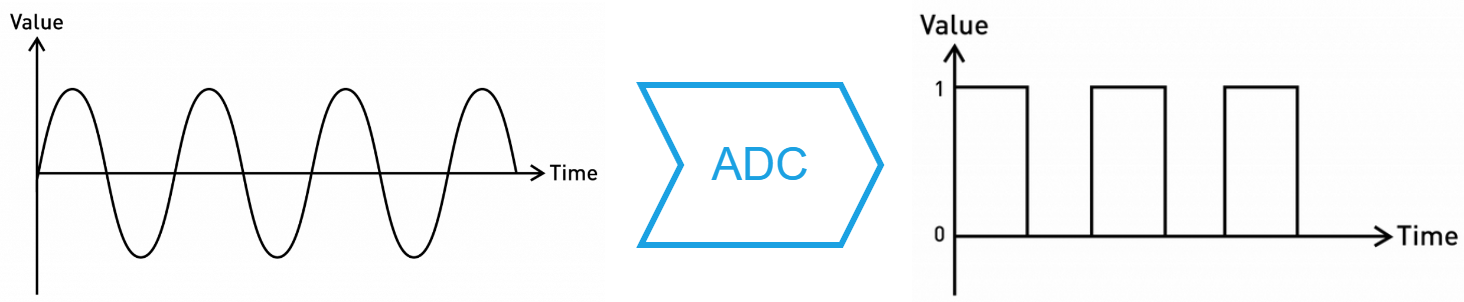
\includegraphics[width=1.0\textwidth]{images/08_durchfuehrung/interface/Conversion.drawio.png}
	\caption{ADC Conversion}
	\label{fig:conversion}
\end{figure}

Der \textbf{Direct Memory Access (DMA)-Controller} übernimmt anschließend die direkte Übertragung dieser digitalen Werte in den Speicher, konkret in  \mintinline{c}|adcBuffer[NUM_CHANNELS]|.

\begin{figure}[H]
\centering
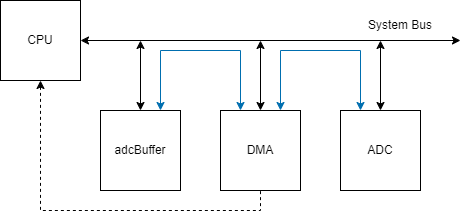
\includegraphics[width=1.0\textwidth]{images/08_durchfuehrung/interface/DMA_ADC_MEM.drawio.png}
\caption{DMA ADC FADER Bus System}
\label{fig:DMA ADC FADER}
\end{figure}

Die DMA ist ein eigener Controller dadurch entlasstet die den Prozessor bei der Datenübertragung direkt zwischen Speicher und Peripheriegeräten.
ADCs sorgen für echtzeitsystemnahe Digitalisierung von analogen Signalen, was eine genaue Messwertverarbeitung ermöglicht. Potentiometer bieten eine benutzerfreundliche Anpassungsmöglichkeiten für Spannungswerte. Das Bussystem dient dann als eine nahtlose Kommunikation zwischen den Komponenten, was zu einer konsistenten und zuverlässigen Datenverarbeitung führt.

\newpage
Die Auswertung und Verarbeitung der Signale erfolgt in der  \mintinline{c}| HAL_ADC_ConvCpltCallback(ADC_HandleTypeDef* hadc)|.

Im laufe der Implementation des ADC könnte man Schwankungen an den Ausgangssignalen des ADCs festellen, was die Genaugigkeit der Potentiometer einstellung beeinflüsste. Diese Schwankungen würden behoben in dem man ein Glättung der Werte eingeführt hat.

Zunächst werden die geglätteten Werte für alle Kanäle des ADC berechnet.

 \inputminted[firstline=121, lastline=135]{c}{../../f401_display_encoder_fader_test/Core/Src/interface.c}

Diese Glättung sorgt dafür, dass die Messwerte stabiler und weniger anfällig für zufällige Schwankungen sind. Anschließend werden die Durchschnittswerte ermittelt. Diese Durchschnittswerte dienen zwei Zwecken: Einerseits werden sie zur Anzeige auf dem Bildschirm verwendet  \mintinline{c}|currentClassPercentADC[]|
, andererseits sind sie für Vergleichsoperationen innerhalb des Sortieralgorithmus von Bedeutung  \mintinline{c}|fm.fader_Class[]|.
 Schließlich wird ein Zeichenarray initialisiert, das später auf dem Display angezeigt wird.\mintinline{c}|faderProzent[0]|.
 
Eine andere möglichkeit des Spannungs inkonsitenz könnte mit Kondensatoren umgesetzt werden was jedoch nicht umgesetzt würde aus zeitlichen Gründen.

\subsubsection{Display, SD1306 Treiber und I2C}

Das Display ist die zentrale Komponente des Interfaces, da es visuelles Feedback auf die Benutzerinteraktionen bietet. Die Kommunikation zwischen dem Nucleo F401RE-Mikrocontroller und dem Display erfolgt über das I2C-Protokoll. Der Mikrocontroller übernimmt die Rolle des Masters, der den Bus steuert, während das Display als Slave agiert. Die Datenübertragung erfolgt über die beiden I2C-Leitungen: SDA (Datenleitung) und SCL (Taktleitung). Der Master beginnt die Kommunikation mit einer Start-Bedingung, gefolgt von der Übertragung der Adresse des Displays und der entsprechenden Daten in Bytes. Diese Daten werden durch die Taktimpulse auf der SCL-Leitung synchronisiert und auf der SDA-Leitung übertragen und bestätigt. Die Kommunikation endet mit einer Stop-Bedingung. Das I2C-Protokoll ermöglicht eine effiziente und koordinierte Datenübertragung zwischen der MCU und dem Display.

Die Ansteuerung des Displays erfolgt über den SD1306-Treiber, der als Schnittstelle zwischen dem Mikrocontroller Nucleo F401RE und dem LCD-Display fungiert. Dieser Treiber ermöglicht die Kommunikation und Befehlsübertragung, indem er die erforderlichen Initialisierungsbefehle an das Display sendet. Für die Unterstützung von SH1103-kompatiblen Bildschirmen würde die Initialisierungssequenz entsprechend angepasst.


\begin{figure}[H]
	\centering
	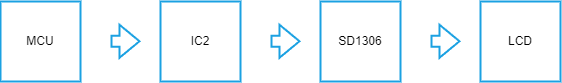
\includegraphics[width=1.0\textwidth]{images/08_durchfuehrung/interface/Display SD1306 Treiber I2C.drawio}
	\caption{Display SD1306 I2C Kommunikation}
	\label{fig:Display SD1306 I2C}
\end{figure}

\newpage

\textcolor{red}{TODO: Begründung der Auswahl des Protokolls}

\textcolor{red}{TODO: Erklärung des Ablaufs mit Codeschnipsel (Aufs wesentliche beziehen)}



\subsubsection{Filesystem}

\textcolor{red}{TODO: Erklärung der Komponente FileManager/File}





